
\documentclass[
	article,			% indica que é um artigo acadêmico
	11pt,				% tamanho da fonte
	oneside,			% para impressão apenas no verso. Oposto a twoside
	a4paper,			% tamanho do papel. 
	english,			% idioma adicional para hifenização
	brazil,				% o último idioma é o principal do documento
	]{abntex2}


\usepackage{cmap}				% Mapear caracteres especiais no PDF
\usepackage{lmodern}			% Usa a fonte Latin Modern
\usepackage[T1]{fontenc}		% Selecao de codigos de fonte.
\usepackage[utf8]{inputenc}		% Codificacao do documento (conversão automática dos acentos)
\usepackage{indentfirst}		% Indenta o primeiro parágrafo de cada seção.
\usepackage{nomencl} 			% Lista de simbolos
\usepackage{color}				% Controle das cores
\usepackage{graphicx}			% Inclusão de gráficos
\usepackage{amsmath}
\usepackage{float}
\usepackage{amssymb}

\usepackage[brazilian,hyperpageref]{backref}	 % Paginas com as citações na bibl
\usepackage[alf]{abntex2cite}	% Citações padrão ABNT

\graphicspath{{./img/}}
\renewcommand{\backrefpagesname}{Citado na(s) página(s):~}

\renewcommand{\backref}{}

\renewcommand*{\backrefalt}[4]{
	\ifcase #1 %
		%Nenhuma citação no texto.%
	\or
		Citado na página #2.%
	\else
		Citado #1 vezes nas páginas #2.%
	\fi}%

\titulo{As superfícies quádricas}
\autor{Diego P. da Jornada\thanks{diego.jornada@acad.pucrs.br}}

\definecolor{blue}{RGB}{41,5,195}

\makeatletter
\hypersetup{
		pdftitle={\@title}, 
		pdfauthor={\@author},
    	pdfsubject={Modelo de artigo científico com abnTeX2},
	    pdfcreator={LaTeX with abnTeX2},
		pdfkeywords={abnt}{latex}{abntex}{abntex2}{atigo científico}, 
		colorlinks=true,       		% false: boxed links; true: colored links
    	linkcolor=blue,          	% color of internal links
    	citecolor=blue,        		% color of links to bibliography
    	filecolor=magenta,      		% color of file links
		urlcolor=blue,
		bookmarksdepth=4
}
\makeatother

\makeindex

\setlrmarginsandblock{4cm}{4cm}{*}
\setulmarginsandblock{4cm}{4cm}{*}
\checkandfixthelayout

\setlength{\parindent}{1.3cm}

\setlength{\parskip}{0.2cm}  % tente também \onelineskip

\SingleSpacing

\begin{document}

\frenchspacing 

\maketitle

\begin{resumoumacoluna}
    
		Este trabalho apresenta algumas superfícies quádricas bem como suas
		definições e representações no $R^3$.

 \vspace{\onelineskip}
 
 \noindent
\end{resumoumacoluna}

\textual

    \section*{Introdução}

		Dentro do escopo da disciplina de \emph{Geometria Analítica} o terceiro
		trabalho pode ser resumido da seguinte maneira: deve-se descrever as
		seguintes superfícies:  Elipsóides, Hiperbolóides e Parabolóides. Além
		das descrições também serão apresentados exemplos gráficos destas
		superfícies.

		O gráfico de uma equação no $R^3$ é chamado de superfície. Uma
		superfície quádrica é representada por uma equação do segundo grau, cuja
		forma geral é $ ax^2 + by^2 + cz^2 + dxy + exz + fyz + gx + hy + iz + j
		= 0$ onde os coeficientes \emph{a}, \emph{b}, \emph{...} e \emph{j} são
		números reais de forma que pelo menos um dos coeficientes \emph{a},
		\emph{b}, \emph{c}, \emph{d}, \emph{e} e \emph{f} é diferente de zero.

    \section{Elipsóides}

		Um elipsóide é uma superfície descrita pelo movimento de uma elipse em
		torno de um eixo, tendo \emph{a, b} e \emph{c} como medidas dos semi
		eixos. Ao girarmos essa elipse em tonor do eixo $Oy$, por exemplo,
		obtemos o \emph{elipsóide de revolução}, caso o centro seja a origem
		então o elipsóide é definido pela Equação ~\ref{elip:geral}.

		\begin{equation}\label{elip:geral}
			\frac{x^2}{a^2}+\frac{y^2}{b^2}+\frac{z^2}{c^2}=1
		\end{equation}

		Na Equação \ref{elip:geral} \emph{a, b} e \emph{c}, são os tamanhos dos
		semi eixos. Se o centro de um elipsóide é o ponto \emph{(h, k, l)} e
		seus eixos forem paralelos aos eixos coordenados pela Equação
		~\ref{elip:desloc}.

		\begin{equation}\label{elip:desloc}
			\frac{(x^2-h)}{a^2}+\frac{(y^2-h)}{b^2}+\frac{(z^2-1)}{c^2}=1
		\end{equation}


		\subsection{Equação Pamétrica}

		A Equação paramétrica do elipsóide pode ser observado na
		Equação~\ref{elip:param}. foram definidos intervalo a \emph{u} e
		\emph{v} para serem usados na representação do elipsóide no $R^3$.
		
		\begin{equation}\label{elip:param}
			\begin{cases}
				x = a\ cos(u) sen(v) &~\\
				y = b\ cos(u) sen(v) &~\\
				z = c\ cos(v) 
			\end{cases}
		\end{equation}


		\subsection{Representação}

		Na Figura~\ref{img:elip} pode ser observado um elipsóide gerado a partir
		da Equação~\ref{elip:param}, de forma que $u\in[-\pi,\pi]$ e
		$v\in[-\frac{\pi}{2}, \frac{\pi}{2}]$.

		\begin{figure}[H]
			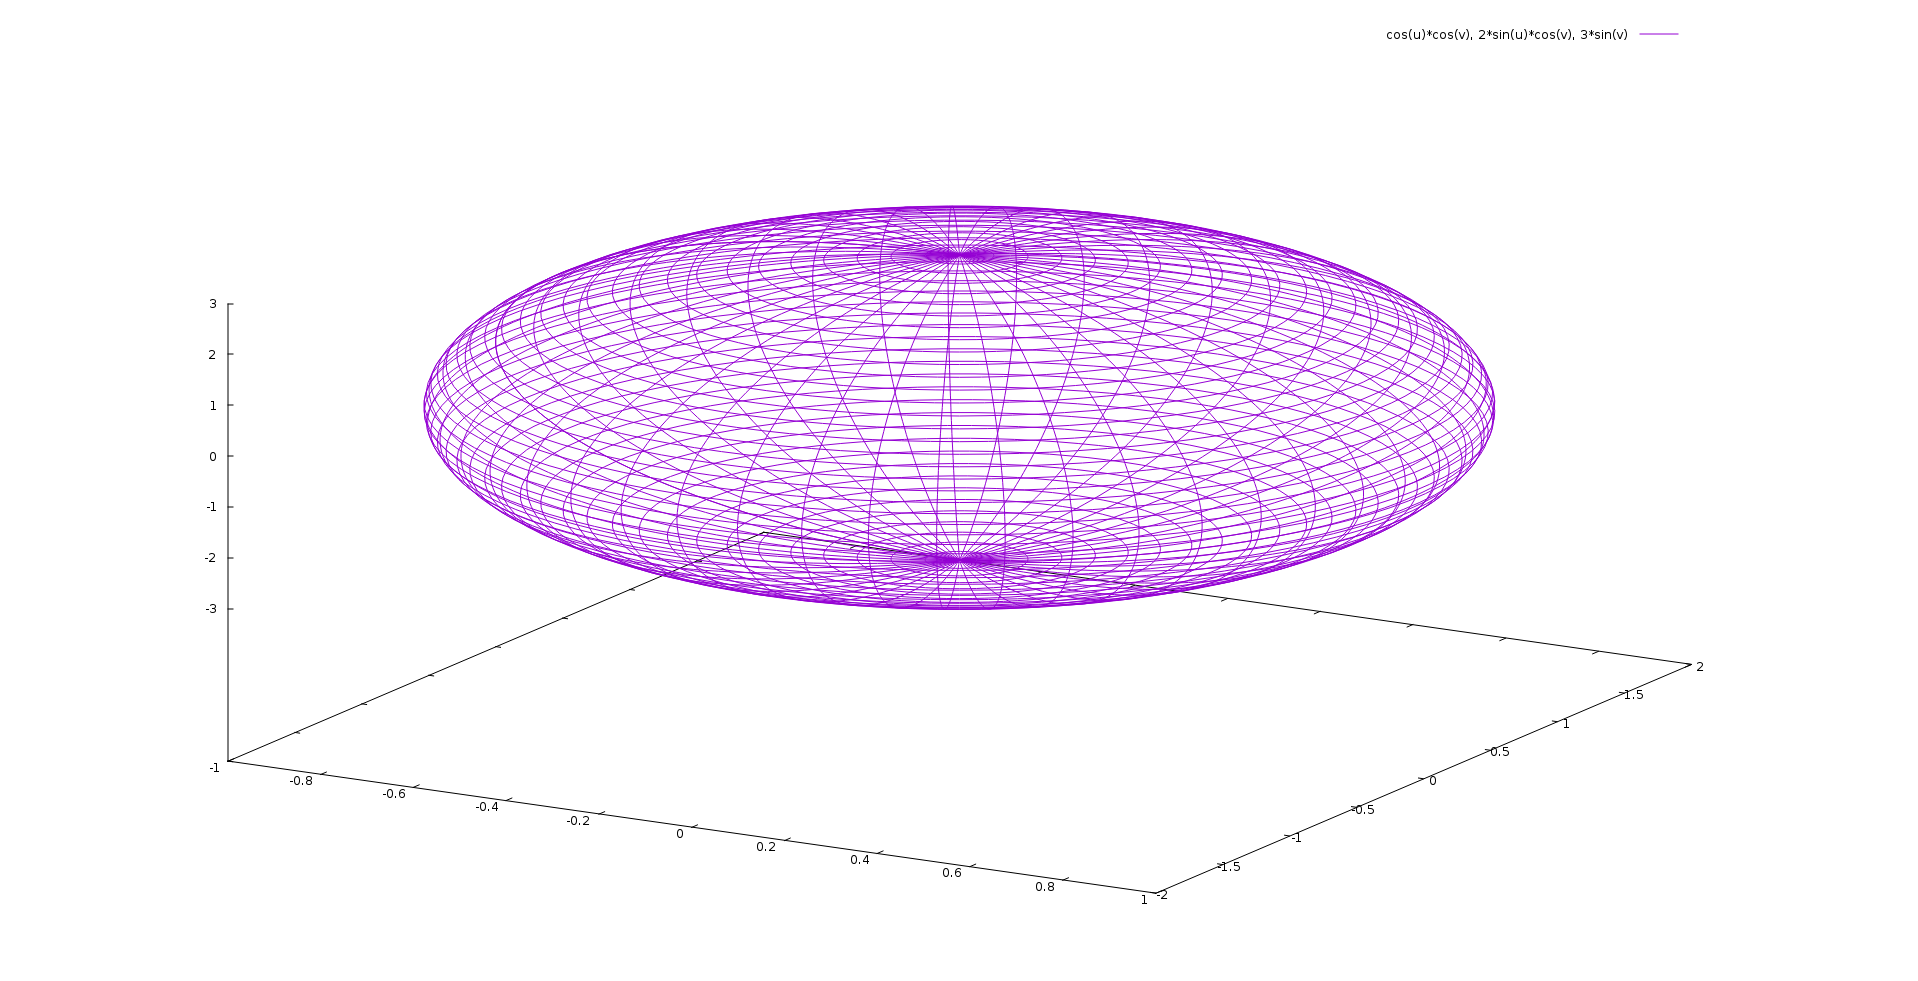
\includegraphics[width=\textwidth,keepaspectratio]{ellipsoid.png}
			\caption{Elipsóide}
			\label{img:elip}
		\end{figure}

	\section{Hiperbolóides} 

		Um hiperbolóide é uma superfície que poder ter uma ou duas folhas. O
		hiperbolóide de uma folha é obtido rotacionando uma hiperbole
		perpendicular ao foco, enquanto o o de duas folhas é botido apartir da
		rotação paralela a uma reta que passa pelo foco.

		\subsection{Hiperbolóide de uma folha}

		A Equação~\ref{hipum:geral} que representa o hiperbolóide de uma
		folha quando seu centro é a origem.

		\begin{equation}\label{hipum:geral}
			\frac{x^2}{a^2}+\frac{y^2}{a^2}-\frac{z^2}{c^2}=1
		\end{equation}


		A Equação~\ref{hipum:param} é a definição paramétrica do hiperbolóide
		de uma folha.

		\begin{equation}\label{hipum:param}
			\begin{cases}
				x = a\ \sqrt{1 + u^2} cos v~\\
				y = a\ \sqrt{1 + u^2} sen v~\\
				z = cu
			\end{cases}
		\end{equation}

		\subsection{Hiperbolóide de duas folhas}

		A Equação~\ref{hipdois:geral} que representa o hiperbolóide de duas
		folhas quando seu centro é a origem.

		\begin{equation}\label{hipdois:geral}
			\frac{x^2}{a^2}+\frac{y^2}{a^2}-\frac{z^2}{c^2}=-1
		\end{equation}


		A Equação~\ref{hipdois:param} é a definição paramétrica do hiperbolóide
		de duas folhas.

		\begin{equation}\label{hipdois:param}
			\begin{cases}
				x = a\ sin(h)\ u cos(v)&~\\
				y = a\ sin(h)\ u sen(v)&~\\
				z = c\ cos(h) u~\\
			\end{cases}
		\end{equation}

		\subsection{Representação}

		A Figure~\ref{img:hip} apresenta um hiperbolóide de uma folha construido a partir da
		equação, onde $u \in[-\pi:\pi]$ e $v\in\mathbb{R}$.

		\begin{figure}[H]
			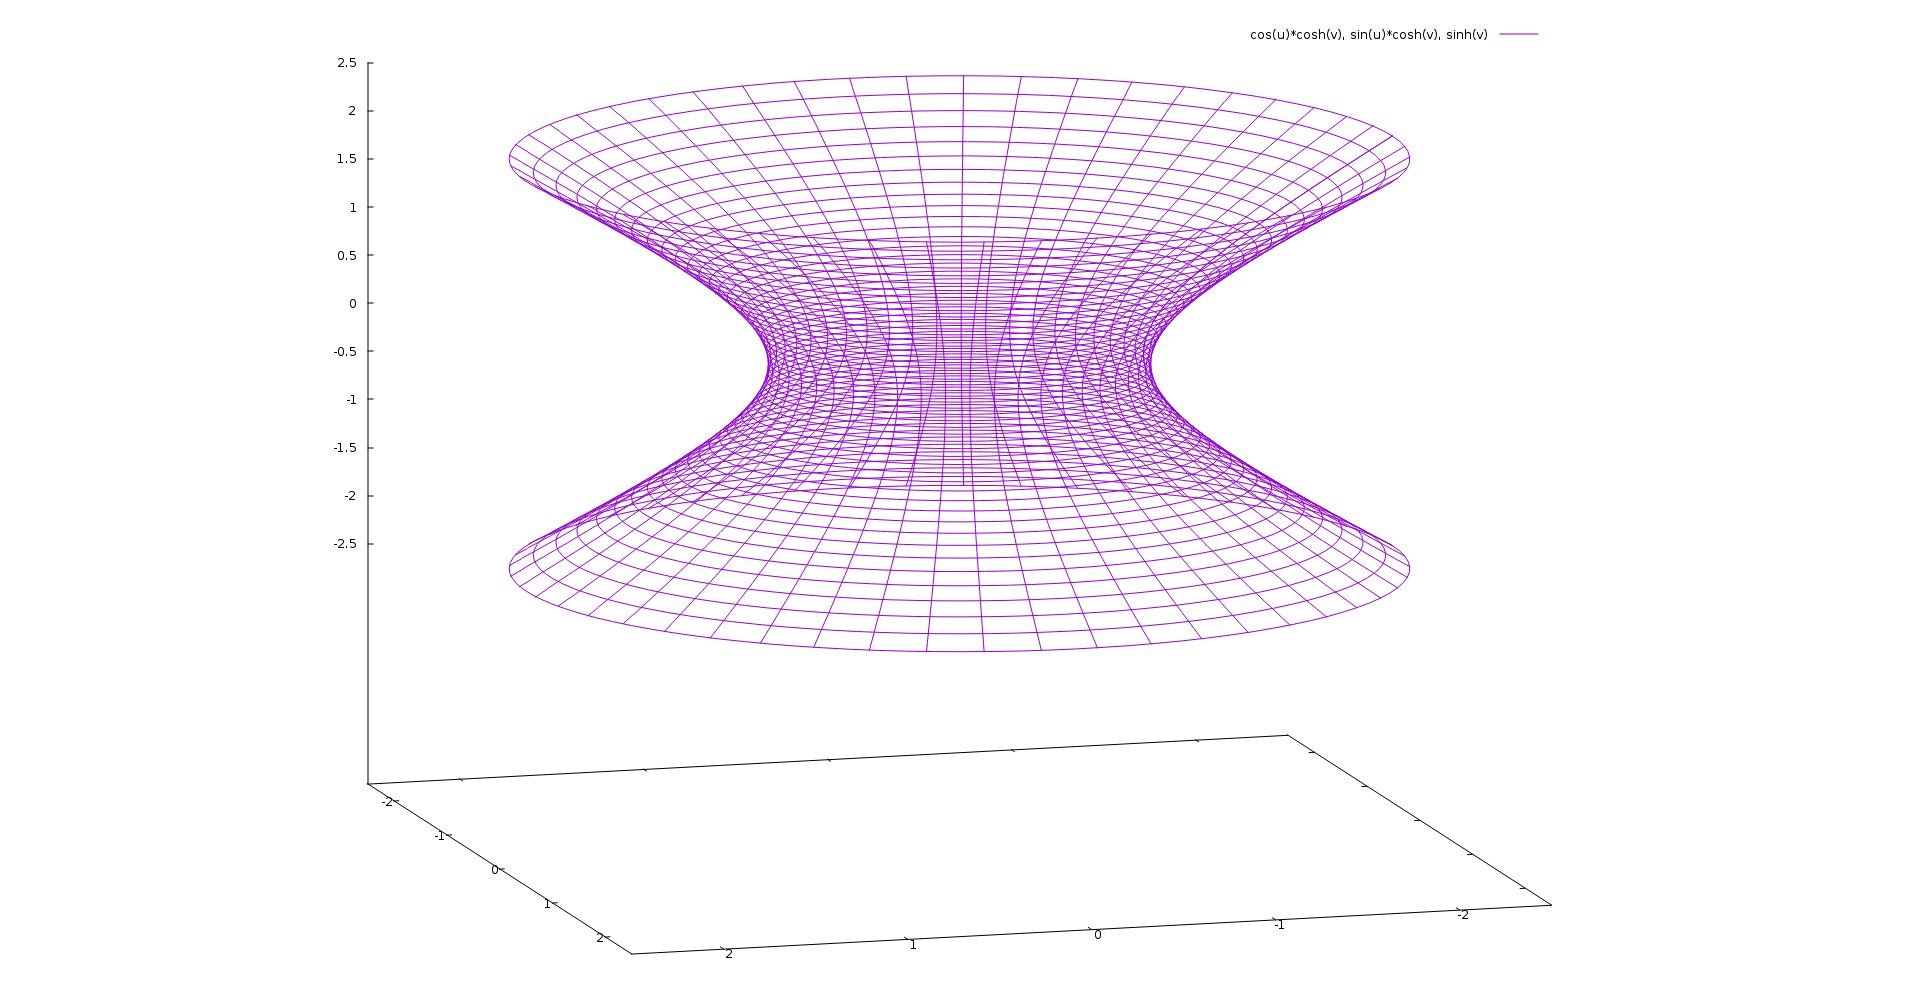
\includegraphics[width=\textwidth,keepaspectratio]{hyperboloid.png}
			\caption{Hiperbolóide}
			\label{img:hip}
		\end{figure}

	\section{Parabolóides}

		Um parabolóide é uma superfície descrita pelo movimento de uma parábola
		ao longo de uma curva planar em torno de um eixo de rotação . Uma
		parábola é uma curva em duas dimensões em que todos os pontos satisfazem
		a equação $z = b(x+y)^2$. Esta parábola é chamada de geratriz da
		superfície. A equação paramétrica do parabolóide está definido na
		Equação ~\ref{parab:param}

		\begin{equation}\label{parab:param}
			\begin{cases}
				x = a\ \sqrt{\frac{u}{h}} cos v~\\
				y = a\ \sqrt{\frac{u}{h}} sen v~\\
				z = u
			\end{cases}
		\end{equation}

		\subsection{Representação}

		Na figura ~\ref{img:parab} é possível visualizar um parabolóide gerado a
		partir da Equação $x^2 + y^2$,onde $x \in[-2:2], y\in[-2:2]$.
				\begin{figure}[H]
					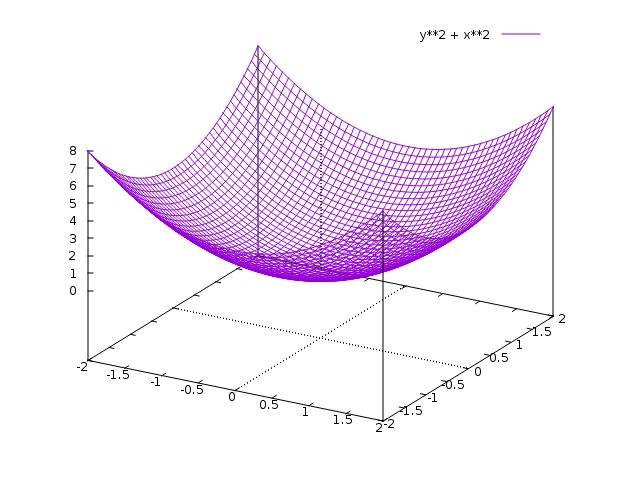
\includegraphics[width=\textwidth,keepaspectratio]{paraboloid.png}
					\caption{Parabolóide}
					\label{img:parab}
				\end{figure}

	\bibliography{bib}
	\nocite{winterle2000vetores}
	\nocite{abbena2006modern}
	\nocite{hilbert1999geometry}
	\end{document}
